\documentclass{assignment}
\UsingEnglish
\ProjectInfos*{Guided Wave Optics}{EE140}{Fall, 2020}{Assignment 1}{Due time : 23:59, Oct 15, 2020 (Thursday)}{陈稼霖}{45875852}
\begin{document}
\begin{prob}
    Consider two planar waveguide show in below: the first one has $n_f=3.5$, $n_c=1$, and $n_s=1.5$, $h=5\mu\mathrm{m}$; the second one has $n_f=2$, $n_c=1$, and $n_s=1.5$, $h=5\mu\mathrm{m}$. Calculate and plot the propagation constants, effective indices, and all the guiding mode profile of TE and TM polarization for both these two waveguides. You can use the software you learned in class or any software you like.
    \begin{figure}[h]
        \centering
        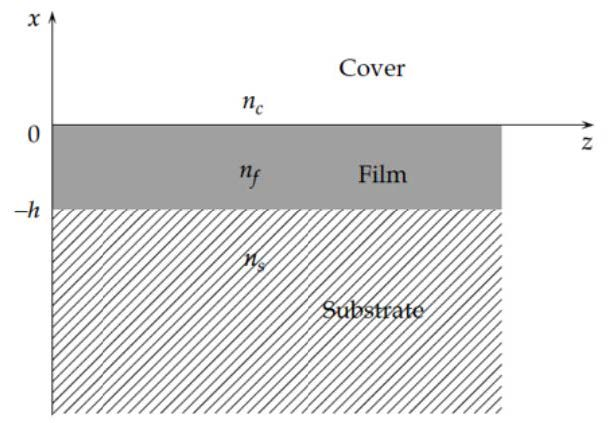
\includegraphics[width=.5\columnwidth]{Assignment-1-Problem-1.jpg}
    \end{figure}
\end{prob}
\begin{sol}
    使用Lumerical软件中的Mode来模拟,设置和结果如下:
    \begin{itemize}
        \item[(1)] \textbf{Materials \& Structures}:设置$x$坐标在$[-5\mu\mathrm{m},0]$范围内、$y$坐标在$[-10\mu\mathrm{m},10\mu\mathrm{m}]$范围内、$z$坐标在$[-0.5\mu\mathrm{m},0.5\mu\mathrm{m}]$范围内、折射率为$3.5$的长方体作为芯层;设置$x$坐标在$[-15\mu\mathrm{m},-5\mu\mathrm{m}]$范围内、$y$坐标在$[-10\mu\mathrm{m},10\mu\mathrm{m}]$范围内、$z$坐标在$[-0.5\mu\mathrm{m},0.5\mathrm{m}]$范围内、折射率为$1.5$的长方体作为衬底. 其余设置默认.

        \textbf{FDE}:设置模拟温度为$300\mathrm{K}$,求解器类型为“2D Z normal”,背景材料折射率为$1$;设置模拟区域的$x$坐标在$[-10\mu\mathrm{m},5\mu\mathrm{m}]$范围内,$y$坐标在$[-5\mu\mathrm{m},5\mu\mathrm{m}]$范围内,$z$坐标为$0$;设置$x_{\min}$和$x_{\max}$处的边界条件为PML,$y_{\min}$和$y_{\max}$处的边界条件为周期性边界条件. 其余设置默认.

        \textbf{Run}:设置波长为$10\mu\mathrm{m}$,在$n=3.5$附近搜寻模式,共得到$7$个模式,其各个参数及模场分布如表\ref{WG-1}所示.
    \begin{longtable}[c]{|c|c|c|c|c|c|c|}
    \caption{}
    \label{WG-1}\\
    \hline
    \begin{tabular}[c]{@{}c@{}}模式\\ 序号\\ \#\end{tabular} &
      \begin{tabular}[c]{@{}c@{}}有效\\ 折射率\\ $N$\end{tabular} &
      \begin{tabular}[c]{@{}c@{}}传播\\ 常数\\ $\beta$ / $\mu\mathrm{m}^{-1}$\end{tabular} &
      \begin{tabular}[c]{@{}c@{}}模式\\ 类型\end{tabular} &
      \begin{tabular}[c]{@{}c@{}}(对TE模)$e_y(x)$\\ (对TM模)$h_y(x)$\end{tabular} &
      \begin{tabular}[c]{@{}c@{}}(对TE模)$h_x(x)$\\ (对TM模)$e_x(x)$\end{tabular} &
      \begin{tabular}[c]{@{}c@{}}(对TE模)$h_z(x)$\\ (对TM模)$e_z(x)$\end{tabular} \\ \hline
    \endfirsthead
    %
    \multicolumn{7}{c}%
    {{\bfseries Table \thetable\ continued from previous page}} \\
    \hline
    \begin{tabular}[c]{@{}c@{}}模式\\ 序号\\ \#\end{tabular} &
      \begin{tabular}[c]{@{}c@{}}有效\\ 折射率\\ $N$\end{tabular} &
      \begin{tabular}[c]{@{}c@{}}传播\\ 常数\\ $\beta$ / $\mu\mathrm{m}^{-1}$\end{tabular} &
      \begin{tabular}[c]{@{}c@{}}模式\\ 类型\end{tabular} &
      \begin{tabular}[c]{@{}c@{}}(对TE模)$e_y(x)$\\ (对TM模)$h_y(x)$\end{tabular} &
      \begin{tabular}[c]{@{}c@{}}(对TE模)$h_x(x)$\\ (对TM模)$e_x(x)$\end{tabular} &
      \begin{tabular}[c]{@{}c@{}}(对TE模)$h_z(x)$\\ (对TM模)$e_z(x)$\end{tabular} \\ \hline
    \endhead
    %
    1 &
      3.3990 &
      2.1356 &
      TE &
      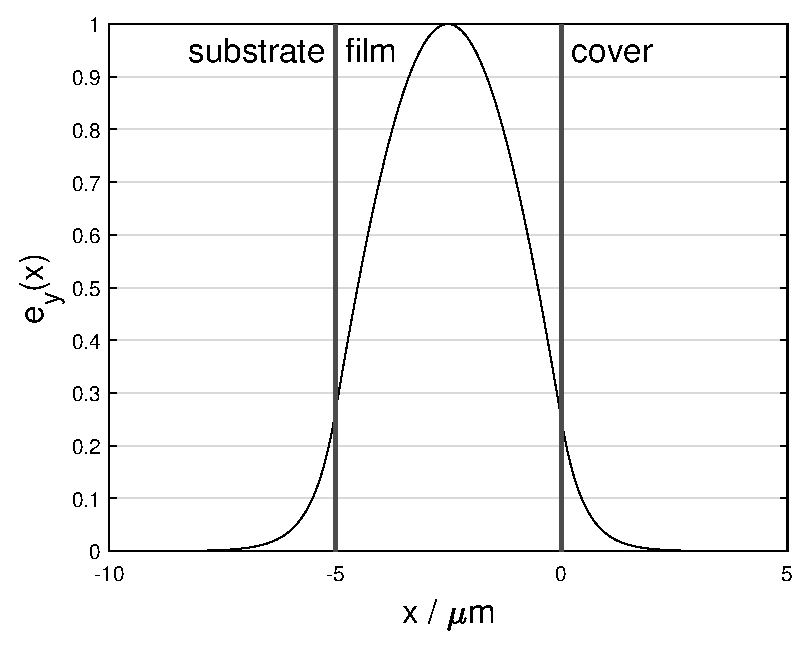
\includegraphics[width=.22\columnwidth]{Assignment-1-Problem-1-WaveGuide-1-ModalAnalysis-Mode-1-Ey.eps} &
      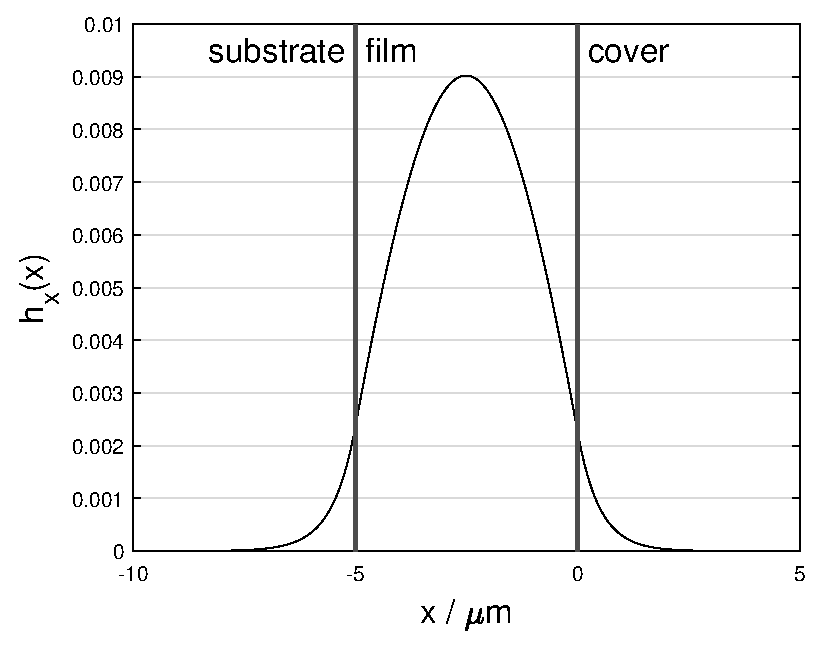
\includegraphics[width=.22\columnwidth]{Assignment-1-Problem-1-WaveGuide-1-ModalAnalysis-Mode-1-Hx.eps} &
      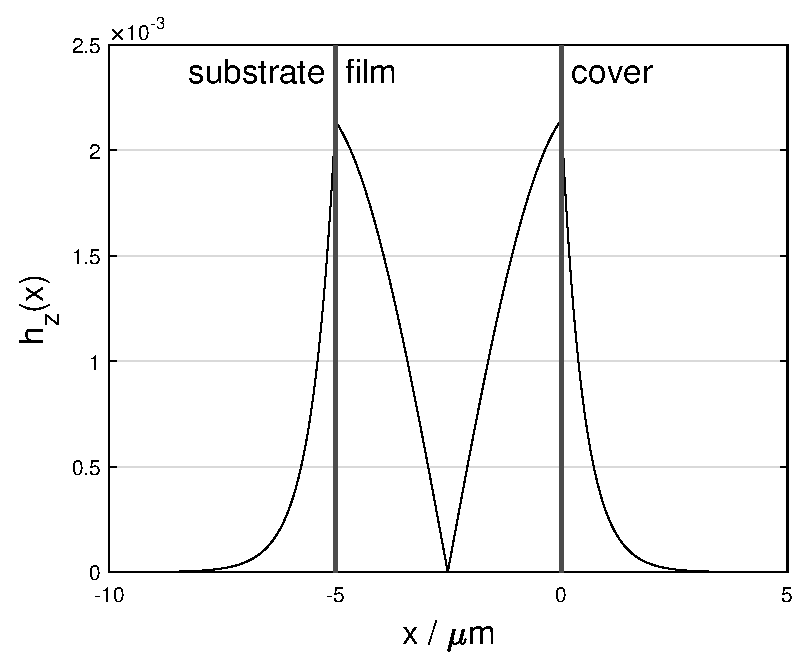
\includegraphics[width=.22\columnwidth]{Assignment-1-Problem-1-WaveGuide-1-ModalAnalysis-Mode-1-Hz.eps} \\ \hline
    2 &
      3.3620 &
      2.1124 &
      TM &
      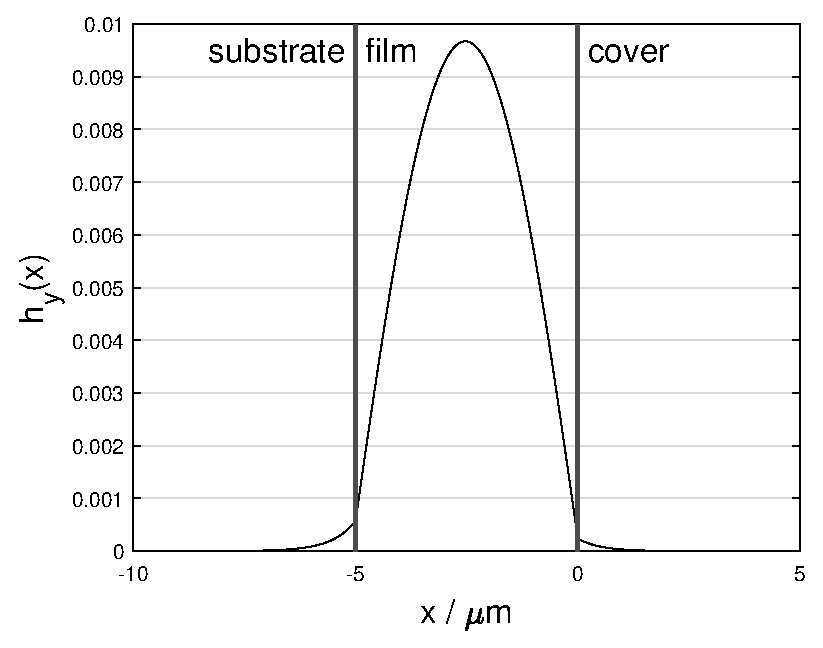
\includegraphics[width=.22\columnwidth]{Assignment-1-Problem-1-WaveGuide-1-ModalAnalysis-Mode-2-Hy.eps} &
      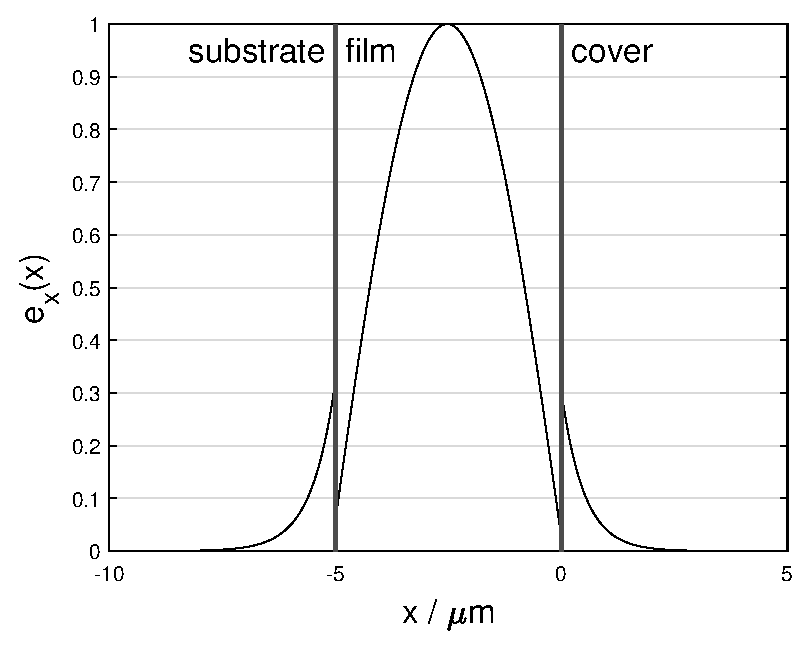
\includegraphics[width=.22\columnwidth]{Assignment-1-Problem-1-WaveGuide-1-ModalAnalysis-Mode-2-Ex.eps} &
      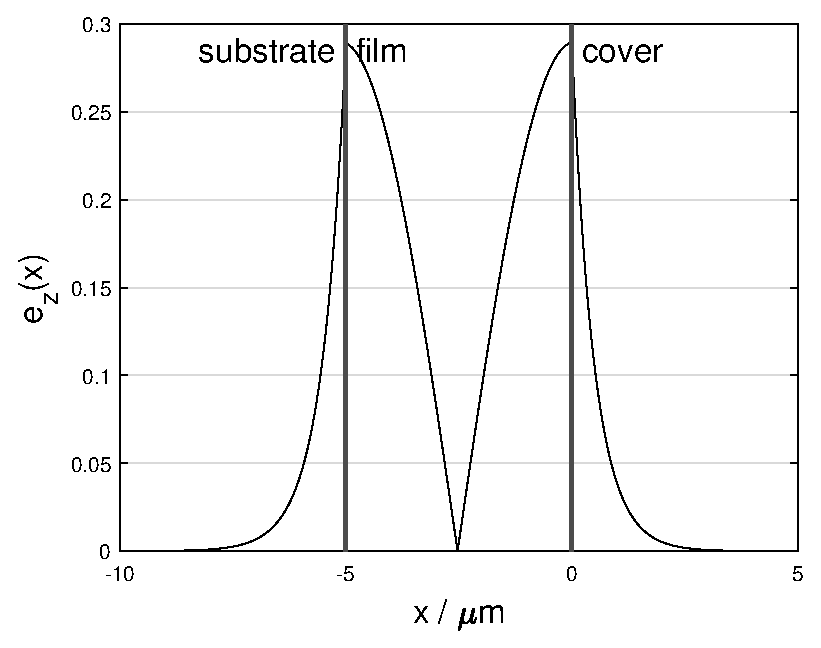
\includegraphics[width=.22\columnwidth]{Assignment-1-Problem-1-WaveGuide-1-ModalAnalysis-Mode-2-Ez.eps} \\ \hline
    3 &
      3.0816 &
      1.9362 &
      TE &
      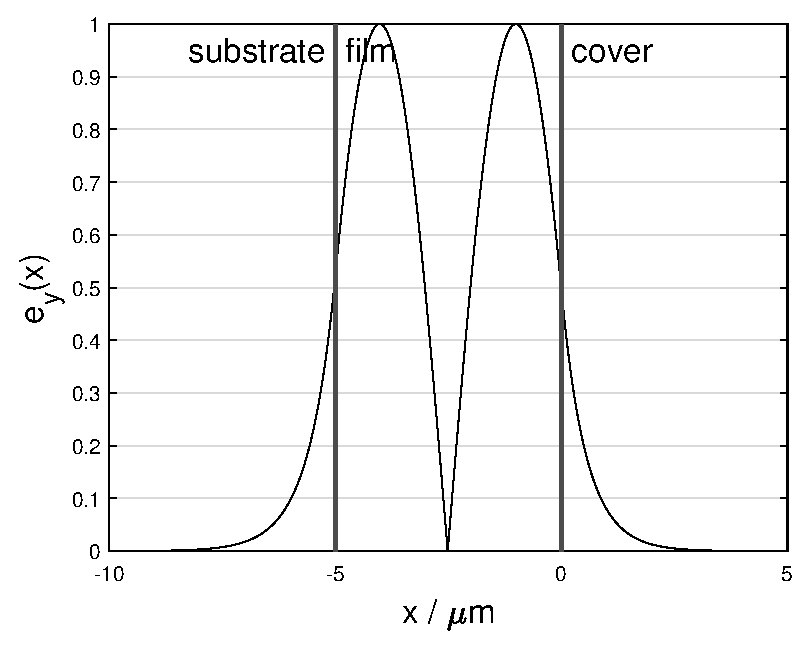
\includegraphics[width=.22\columnwidth]{Assignment-1-Problem-1-WaveGuide-1-ModalAnalysis-Mode-3-Ey.eps} &
      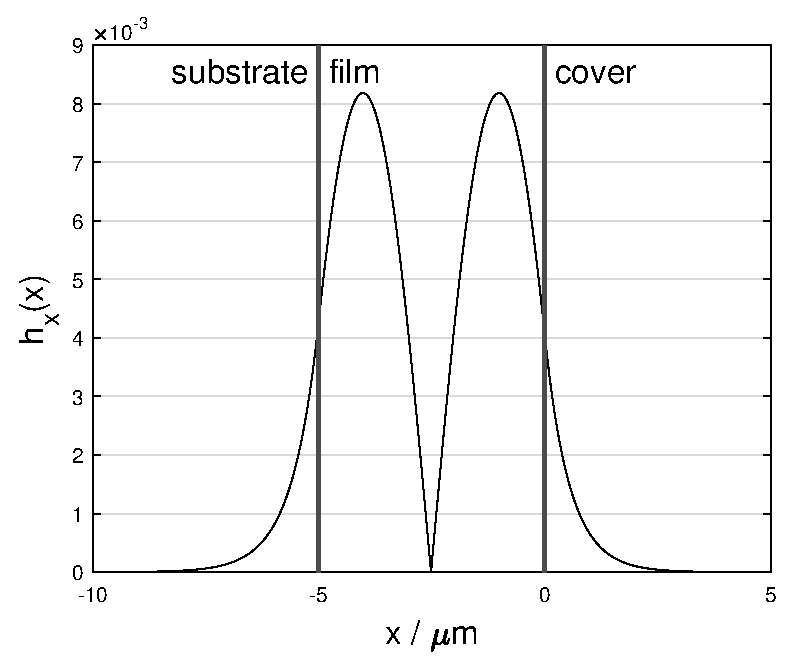
\includegraphics[width=.22\columnwidth]{Assignment-1-Problem-1-WaveGuide-1-ModalAnalysis-Mode-3-Hx.eps} &
      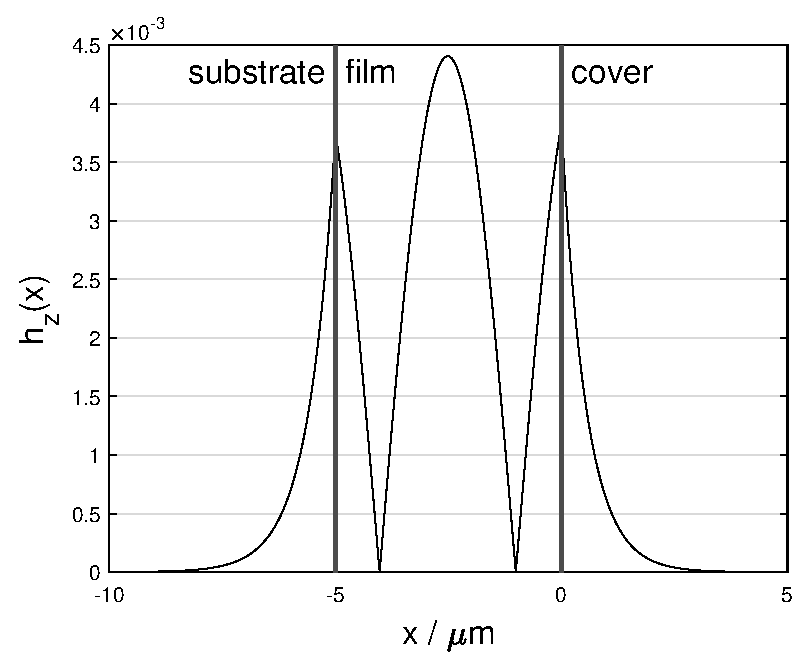
\includegraphics[width=.22\columnwidth]{Assignment-1-Problem-1-WaveGuide-1-ModalAnalysis-Mode-3-Hz.eps} \\ \hline
    4 &
      2.9154 &
      1.8318 &
      TM &
      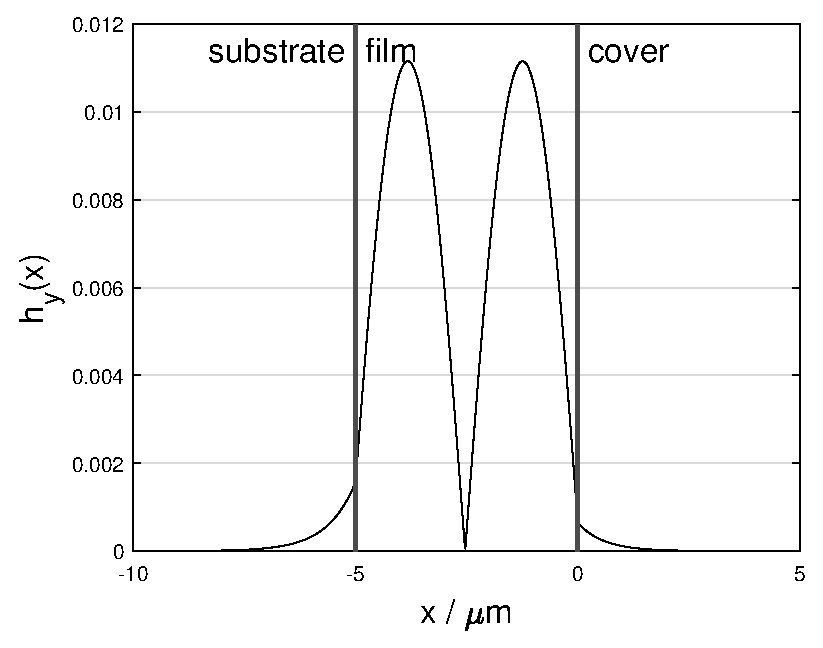
\includegraphics[width=.22\columnwidth]{Assignment-1-Problem-1-WaveGuide-1-ModalAnalysis-Mode-4-Hy.eps} &
      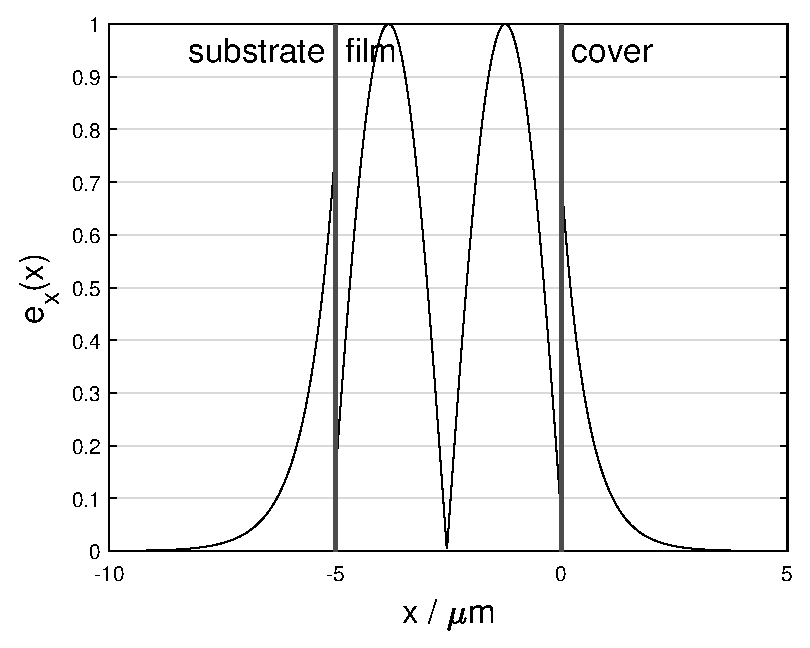
\includegraphics[width=.22\columnwidth]{Assignment-1-Problem-1-WaveGuide-1-ModalAnalysis-Mode-4-Ex.eps} &
      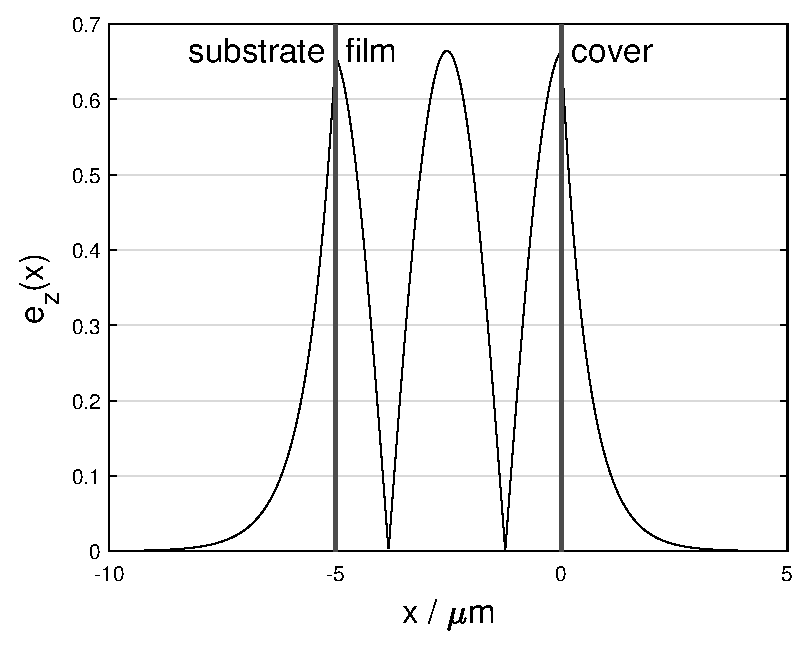
\includegraphics[width=.22\columnwidth]{Assignment-1-Problem-1-WaveGuide-1-ModalAnalysis-Mode-4-Ez.eps} \\ \hline
    5 &
      2.4941 &
      1.5671 &
      TE &
      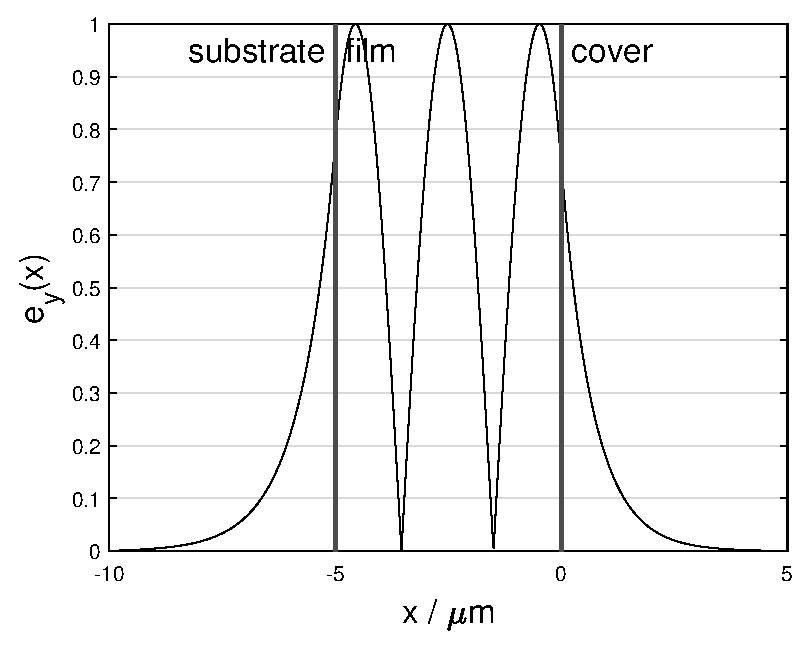
\includegraphics[width=.22\columnwidth]{Assignment-1-Problem-1-WaveGuide-1-ModalAnalysis-Mode-5-Ey.eps} &
      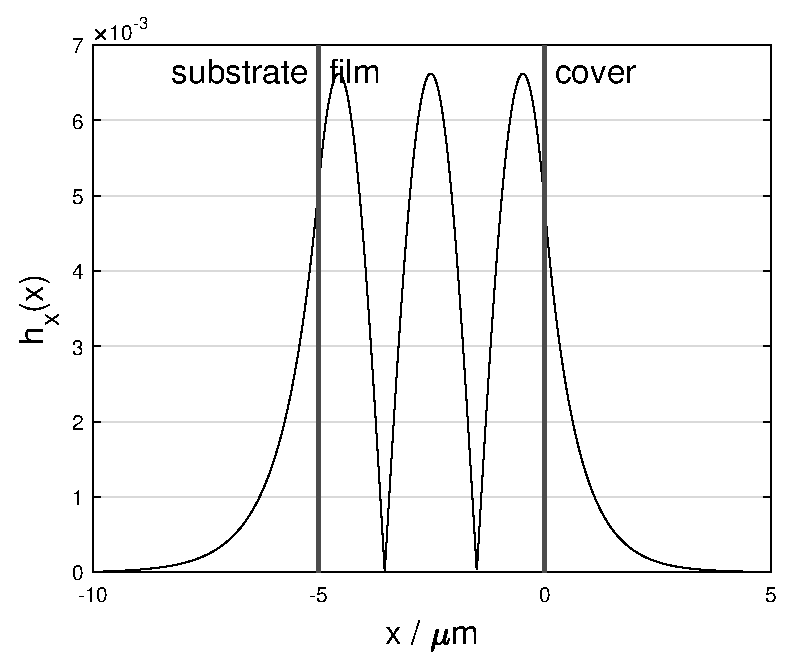
\includegraphics[width=.22\columnwidth]{Assignment-1-Problem-1-WaveGuide-1-ModalAnalysis-Mode-5-Hx.eps} &
      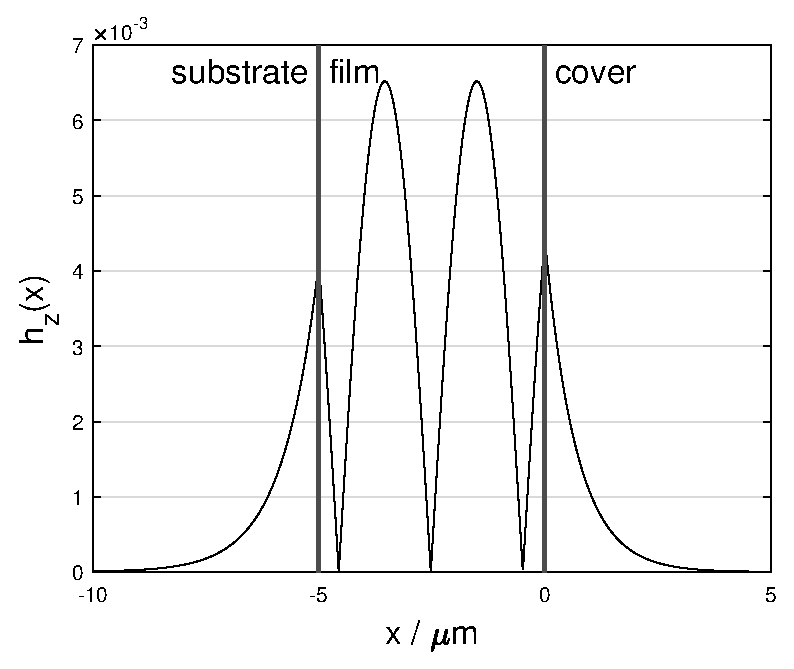
\includegraphics[width=.22\columnwidth]{Assignment-1-Problem-1-WaveGuide-1-ModalAnalysis-Mode-5-Hz.eps} \\ \hline
    6 &
      2.0405 &
      1.2821 &
      TM &
      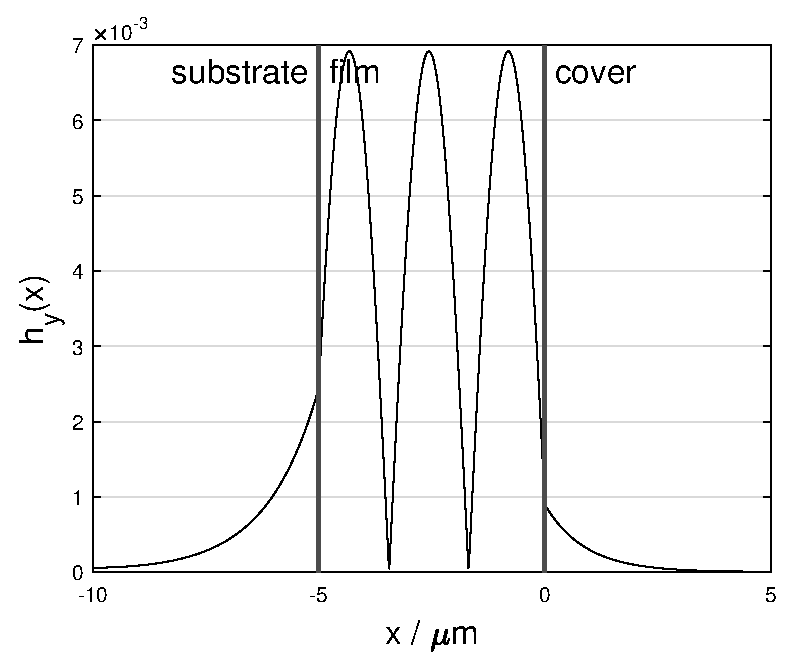
\includegraphics[width=.22\columnwidth]{Assignment-1-Problem-1-WaveGuide-1-ModalAnalysis-Mode-6-Hy.eps} &
      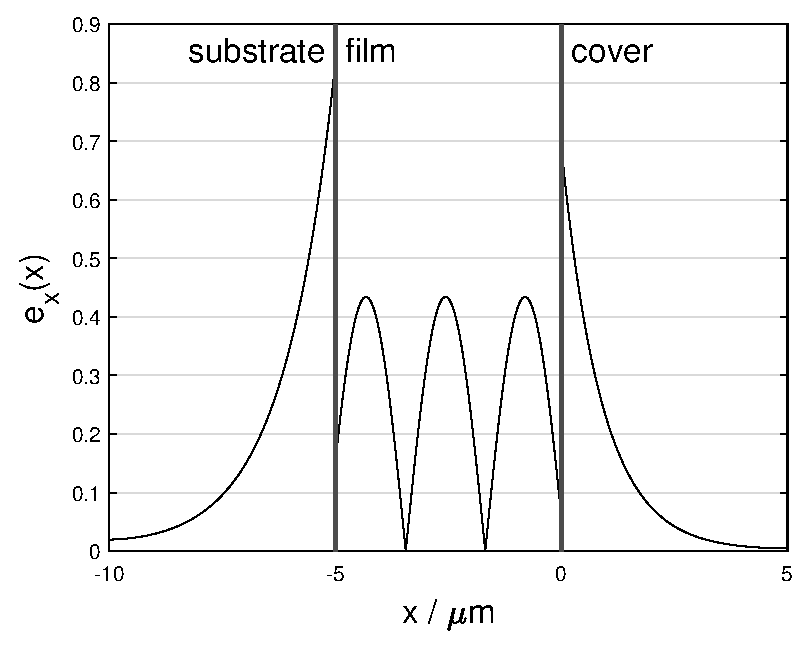
\includegraphics[width=.22\columnwidth]{Assignment-1-Problem-1-WaveGuide-1-ModalAnalysis-Mode-6-Ex.eps} &
      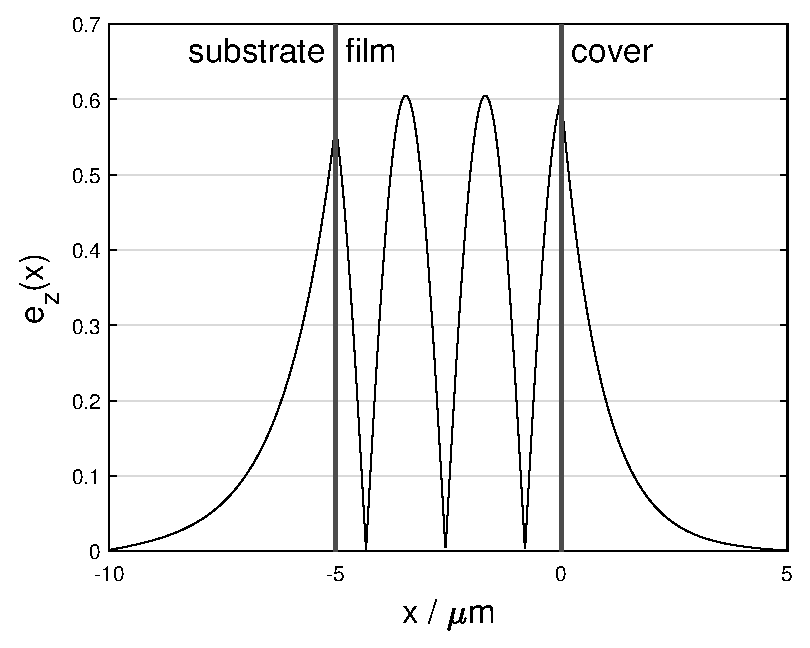
\includegraphics[width=.22\columnwidth]{Assignment-1-Problem-1-WaveGuide-1-ModalAnalysis-Mode-6-Ez.eps} \\ \hline
    7 &
      1.5246 &
      0.9579 &
      TE &
      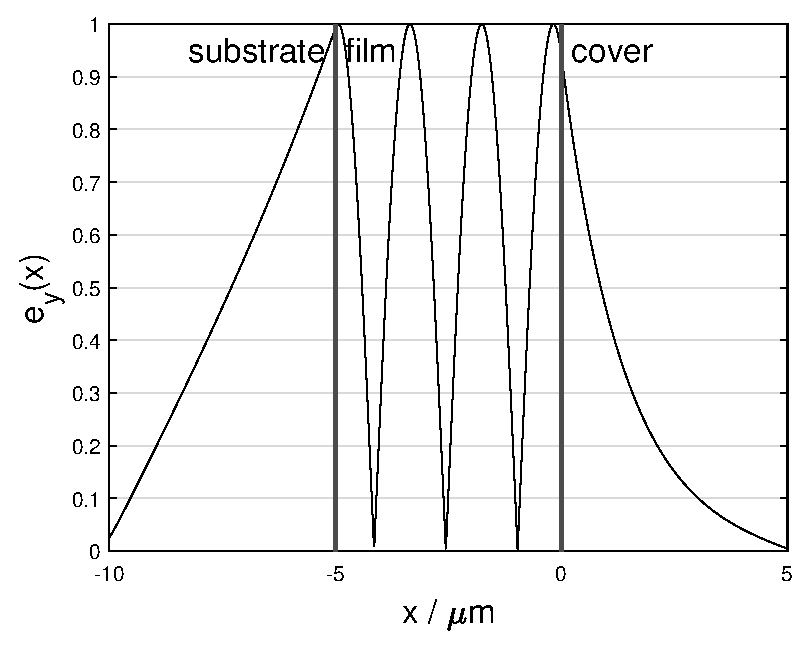
\includegraphics[width=.22\columnwidth]{Assignment-1-Problem-1-WaveGuide-1-ModalAnalysis-Mode-7-Ey.eps} &
      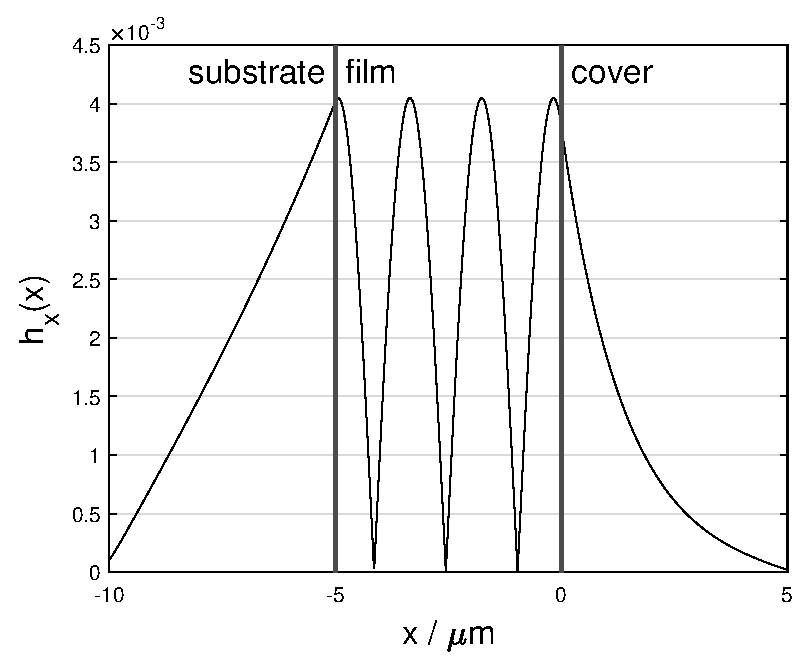
\includegraphics[width=.22\columnwidth]{Assignment-1-Problem-1-WaveGuide-1-ModalAnalysis-Mode-7-Hx.eps} &
      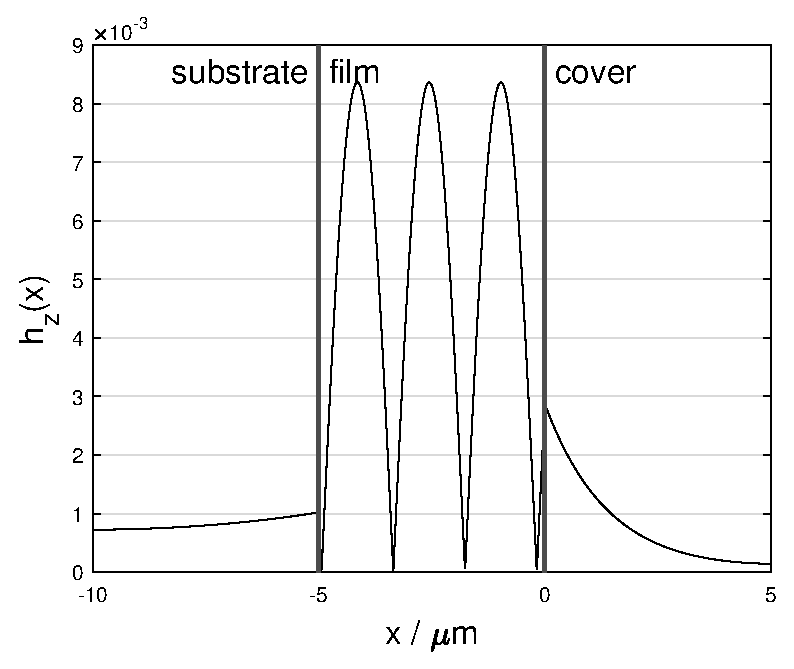
\includegraphics[width=.22\columnwidth]{Assignment-1-Problem-1-WaveGuide-1-ModalAnalysis-Mode-7-Hz.eps} \\ \hline
    \end{longtable}
    \item[(2)] \textbf{Materials \& Structures}:设置$x$坐标在$[-5\mu\mathrm{m},0]$范围内、$y$坐标在$[-10\mu\mathrm{m},10\mu\mathrm{m}]$范围内、$z$坐标在$[-0.5\mu\mathrm{m},0.5\mu\mathrm{m}]$范围内、折射率为$2$的长方体作为芯层;设置$x$坐标在$[-15\mu\mathrm{m},-5\mu\mathrm{m}]$范围内、$y$坐标在$[-10\mu\mathrm{m},10\mu\mathrm{m}]$范围内、$z$坐标在$[-0.5\mu\mathrm{m},0.5\mathrm{m}]$范围内、折射率为$1.5$的长方体作为衬底. 其余设置默认.

    \textbf{FDE}:设置模拟温度为$300\mathrm{K}$,求解器类型为“2D Z normal”,背景材料折射率为$1$;设置模拟区域的$x$坐标在$[-10\mu\mathrm{m},5\mu\mathrm{m}]$范围内,$y$坐标在$[-5\mu\mathrm{m},5\mu\mathrm{m}]$范围内,$z$坐标为$0$;设置$x_{\min}$和$x_{\max}$处的边界条件为PML,$y_{\min}$和$y_{\max}$处的边界条件为周期性边界条件. 其余设置默认.

    \textbf{Run}:设置波长为$5\mu\mathrm{m}$,在$n=2$附近搜寻模式,共得到$6$个模式(虽然计算得到$8$个模式,但是后两个模式中模场被束缚在衬底,有效折射率已小于芯层折射率,这是使用了PML边界条件的缘故,实际并不存在),其各个参数及模场分布如表\ref{WG-2}所示.
    \begin{longtable}[c]{|c|c|c|c|c|c|c|}
    \caption{}
    \label{WG-2}\\
    \hline
    \begin{tabular}[c]{@{}c@{}}模式\\ 序号\\ \#\end{tabular} &
      \begin{tabular}[c]{@{}c@{}}有效\\ 折射率\\ $N$\end{tabular} &
      \begin{tabular}[c]{@{}c@{}}传播\\ 常数\\ $\beta$ / $\mu\mathrm{m}^{-1}$\end{tabular} &
      \begin{tabular}[c]{@{}c@{}}模式\\ 类型\end{tabular} &
      \begin{tabular}[c]{@{}c@{}}(对TE模)$e_y(x)$\\ (对TM模)$h_y(x)$\end{tabular} &
      \begin{tabular}[c]{@{}c@{}}(对TE模)$h_x(x)$\\ (对TM模)$e_x(x)$\end{tabular} &
      \begin{tabular}[c]{@{}c@{}}(对TE模)$h_z(x)$\\ (对TM模)$e_z(x)$\end{tabular} \\ \hline
    \endfirsthead
    %
    \multicolumn{7}{c}%
    {{\bfseries Table \thetable\ continued from previous page}} \\
    \hline
    \begin{tabular}[c]{@{}c@{}}模式\\ 序号\\ \#\end{tabular} &
      \begin{tabular}[c]{@{}c@{}}有效\\ 折射率\\ $N$\end{tabular} &
      \begin{tabular}[c]{@{}c@{}}传播\\ 常数\\ $\beta$ / $\mu\mathrm{m}^{-1}$\end{tabular} &
      \begin{tabular}[c]{@{}c@{}}模式\\ 类型\end{tabular} &
      \begin{tabular}[c]{@{}c@{}}(对TE模)$e_y(x)$\\ (对TM模)$h_y(x)$\end{tabular} &
      \begin{tabular}[c]{@{}c@{}}(对TE模)$h_x(x)$\\ (对TM模)$e_x(x)$\end{tabular} &
      \begin{tabular}[c]{@{}c@{}}(对TE模)$h_z(x)$\\ (对TM模)$e_z(x)$\end{tabular} \\ \hline
    \endhead
    %
    1 &
      1.9572 &
      2.4595 &
      TE &
      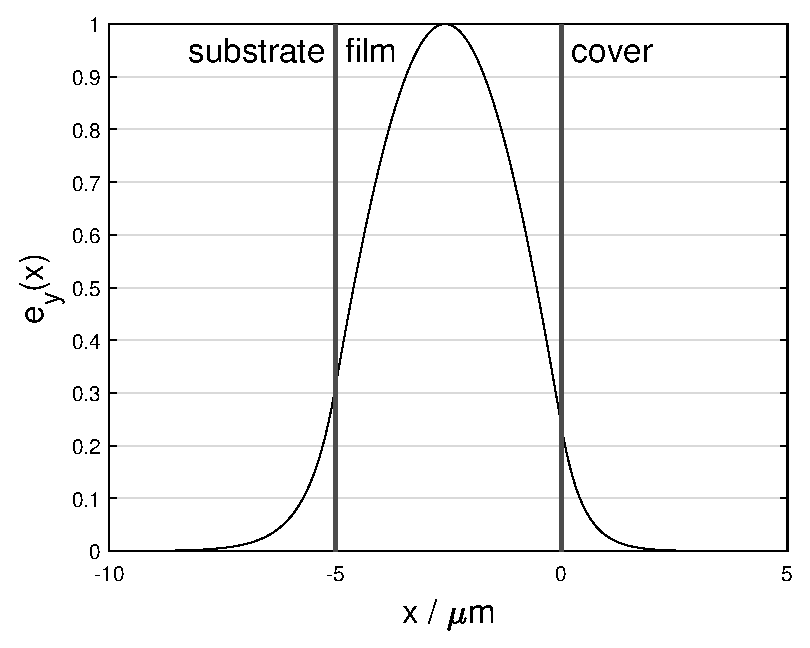
\includegraphics[width=.22\columnwidth]{Assignment-1-Problem-1-WaveGuide-2-ModalAnalysis-Mode-1-Ey.eps} &
      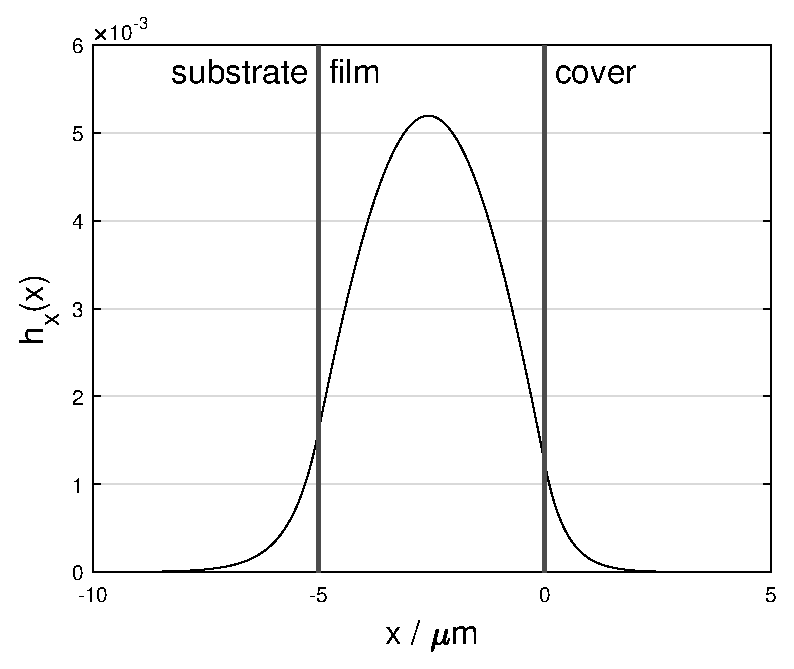
\includegraphics[width=.22\columnwidth]{Assignment-1-Problem-1-WaveGuide-2-ModalAnalysis-Mode-1-Hx.eps} &
      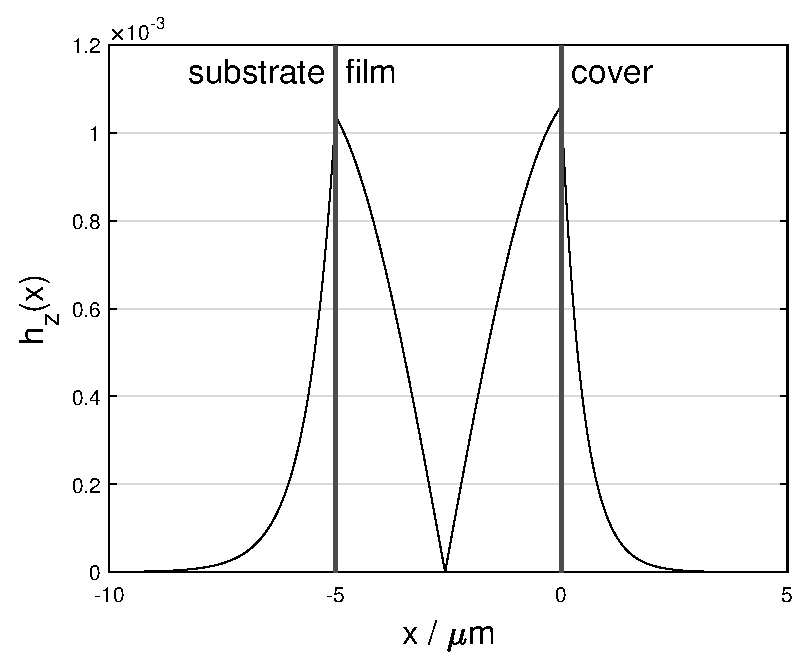
\includegraphics[width=.22\columnwidth]{Assignment-1-Problem-1-WaveGuide-2-ModalAnalysis-Mode-1-Hz.eps} \\ \hline
    2 &
      1.9472 &
      2.4469 &
      TM &
      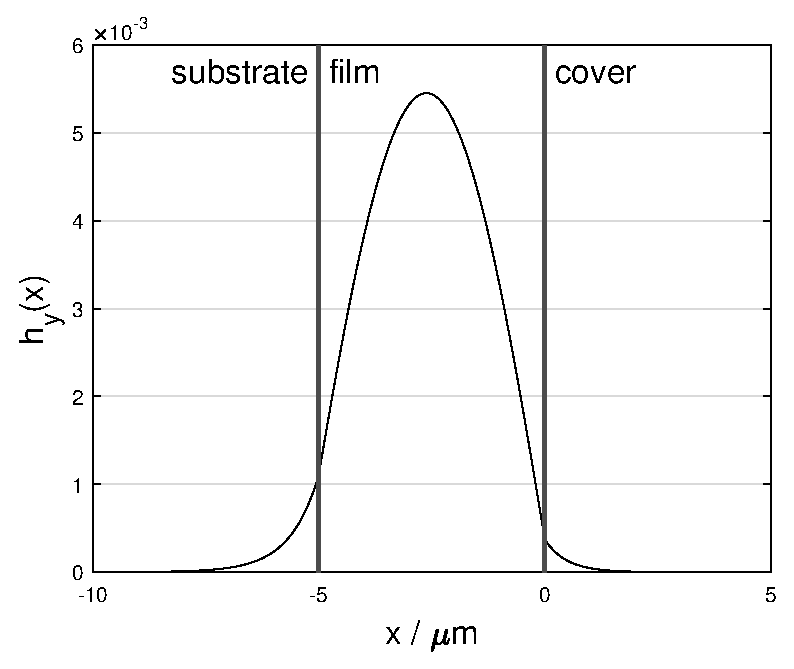
\includegraphics[width=.22\columnwidth]{Assignment-1-Problem-1-WaveGuide-2-ModalAnalysis-Mode-2-Hy.eps} &
      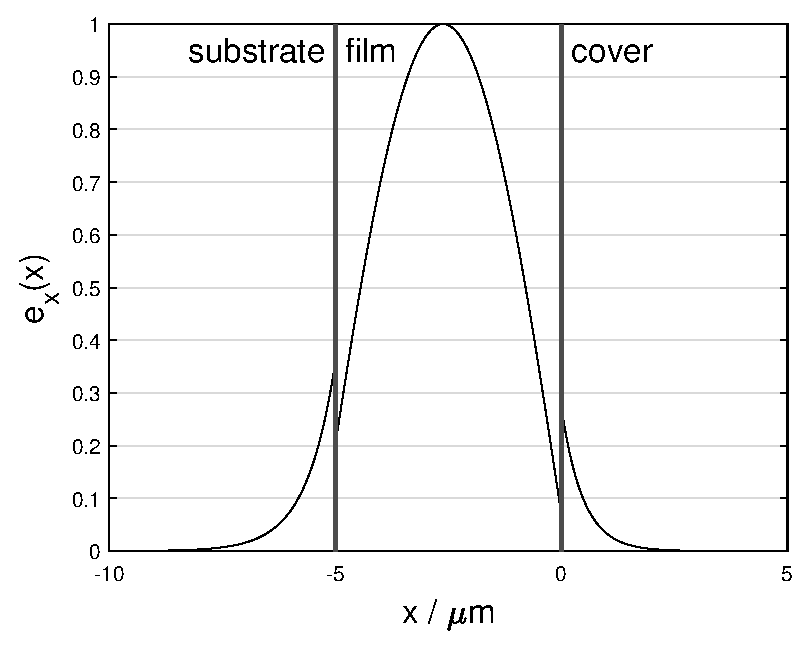
\includegraphics[width=.22\columnwidth]{Assignment-1-Problem-1-WaveGuide-2-ModalAnalysis-Mode-2-Ex.eps} &
      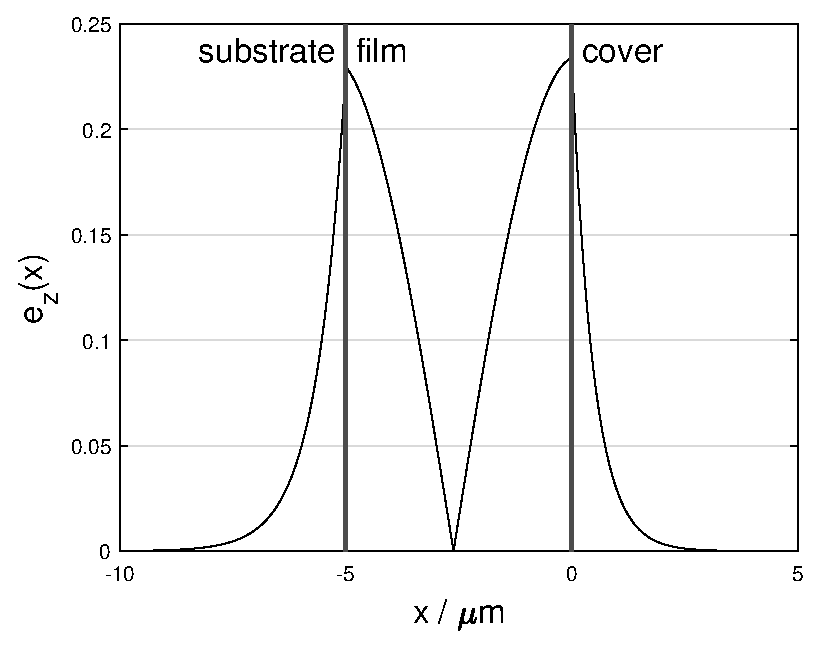
\includegraphics[width=.22\columnwidth]{Assignment-1-Problem-1-WaveGuide-2-ModalAnalysis-Mode-2-Ez.eps} \\ \hline
    3 &
      1.8259 &
      2.2945 &
      TE &
      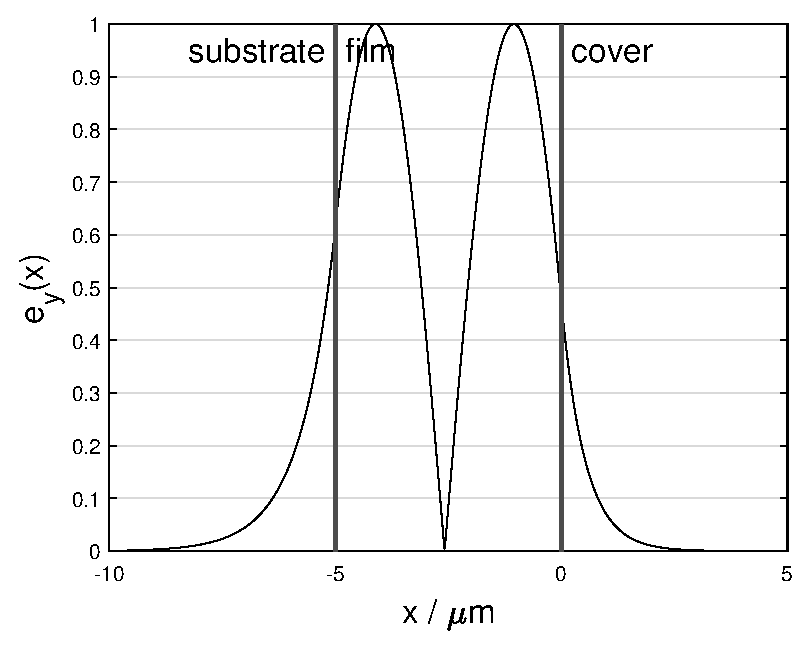
\includegraphics[width=.22\columnwidth]{Assignment-1-Problem-1-WaveGuide-2-ModalAnalysis-Mode-3-Ey.eps} &
      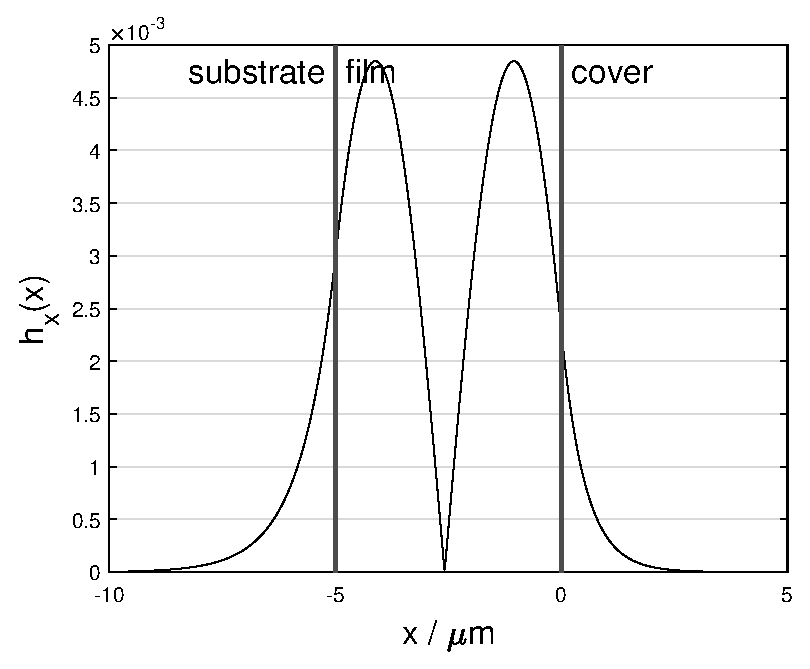
\includegraphics[width=.22\columnwidth]{Assignment-1-Problem-1-WaveGuide-2-ModalAnalysis-Mode-3-Hx.eps} &
      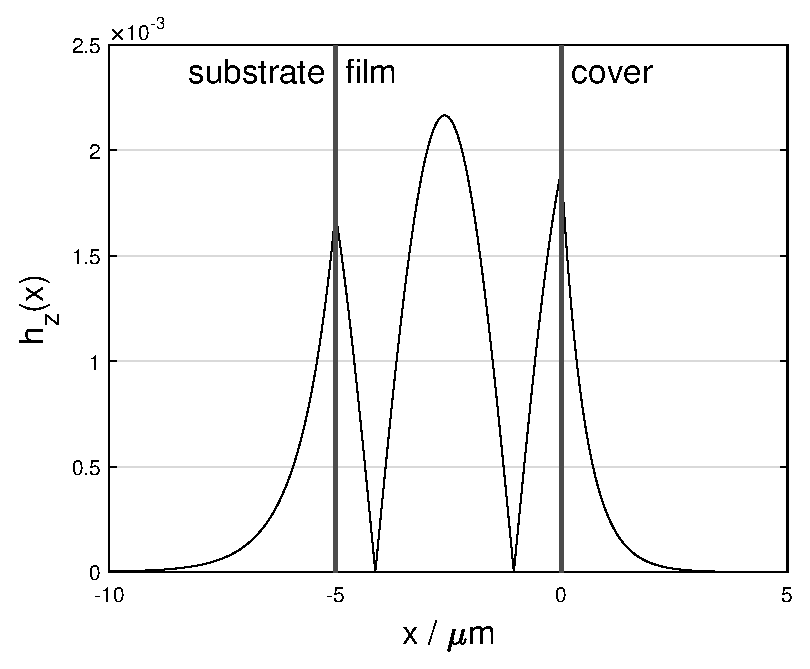
\includegraphics[width=.22\columnwidth]{Assignment-1-Problem-1-WaveGuide-2-ModalAnalysis-Mode-3-Hz.eps} \\ \hline
    4 &
      1.7863 &
      2.2448 &
      TM &
      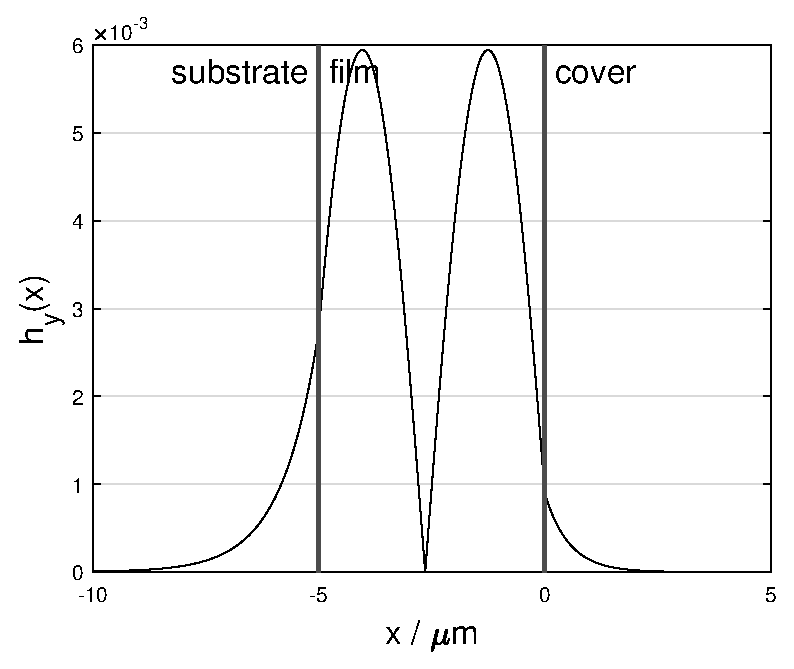
\includegraphics[width=.22\columnwidth]{Assignment-1-Problem-1-WaveGuide-2-ModalAnalysis-Mode-4-Hy.eps} &
      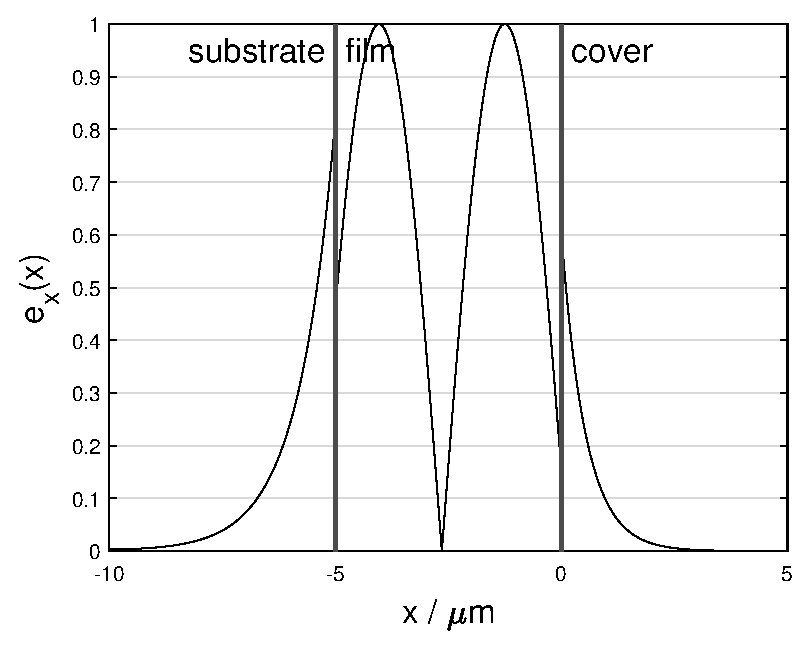
\includegraphics[width=.22\columnwidth]{Assignment-1-Problem-1-WaveGuide-2-ModalAnalysis-Mode-4-Ex.eps} &
      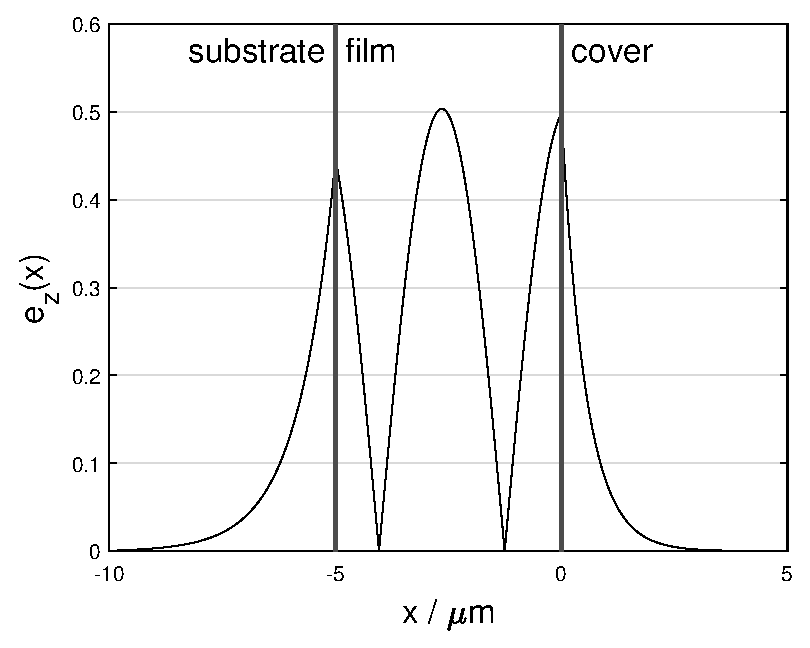
\includegraphics[width=.22\columnwidth]{Assignment-1-Problem-1-WaveGuide-2-ModalAnalysis-Mode-4-Ez.eps} \\ \hline
    5 &
      1.6014 &
      2.0123 &
      TE &
      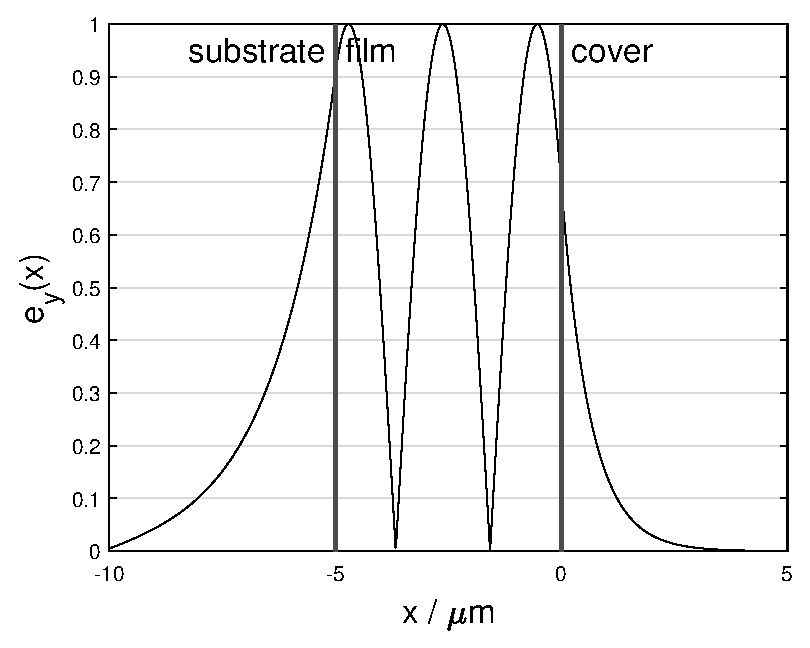
\includegraphics[width=.22\columnwidth]{Assignment-1-Problem-1-WaveGuide-2-ModalAnalysis-Mode-5-Ey.eps} &
      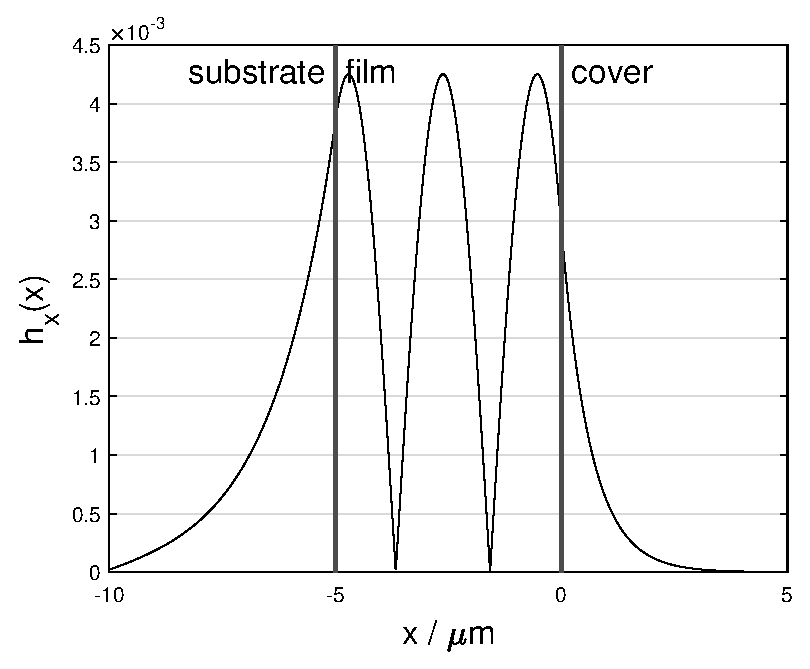
\includegraphics[width=.22\columnwidth]{Assignment-1-Problem-1-WaveGuide-2-ModalAnalysis-Mode-5-Hx.eps} &
      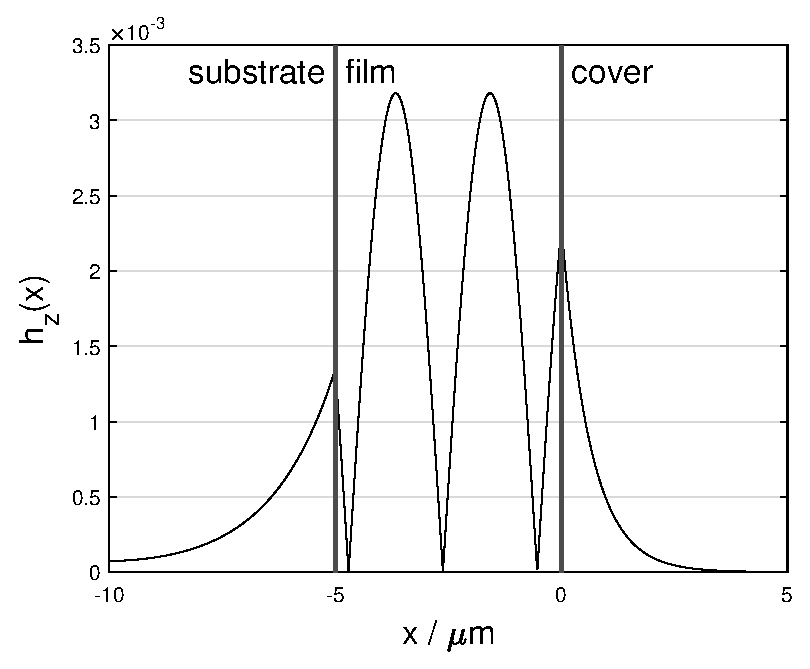
\includegraphics[width=.22\columnwidth]{Assignment-1-Problem-1-WaveGuide-2-ModalAnalysis-Mode-5-Hz.eps} \\ \hline
    6 &
      1.5390 &
      1.9340 &
      TM &
      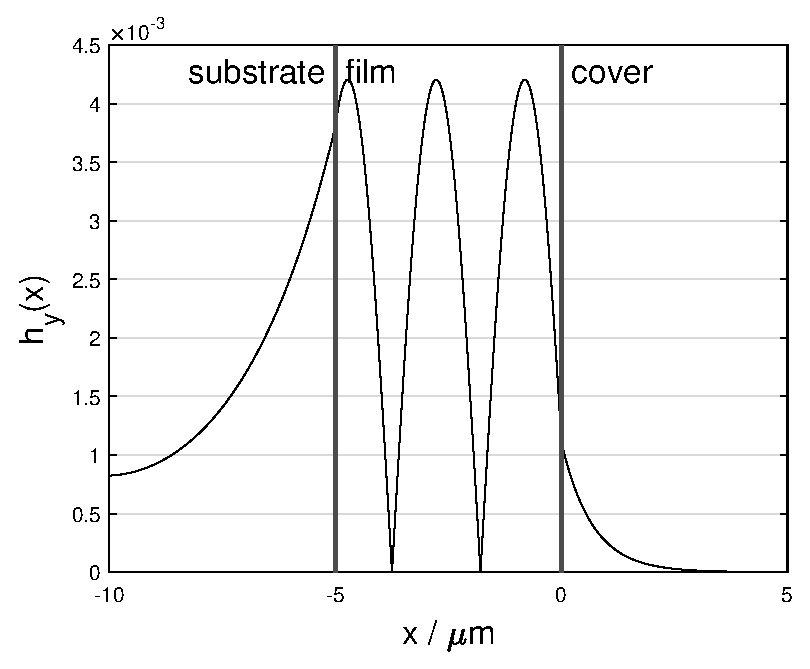
\includegraphics[width=.22\columnwidth]{Assignment-1-Problem-1-WaveGuide-2-ModalAnalysis-Mode-6-Hy.eps} &
      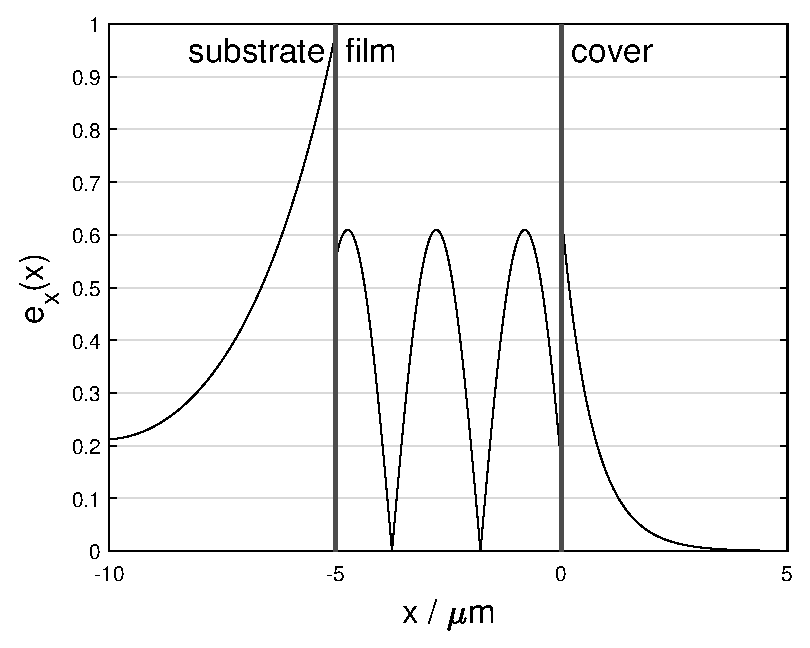
\includegraphics[width=.22\columnwidth]{Assignment-1-Problem-1-WaveGuide-2-ModalAnalysis-Mode-6-Ex.eps} &
      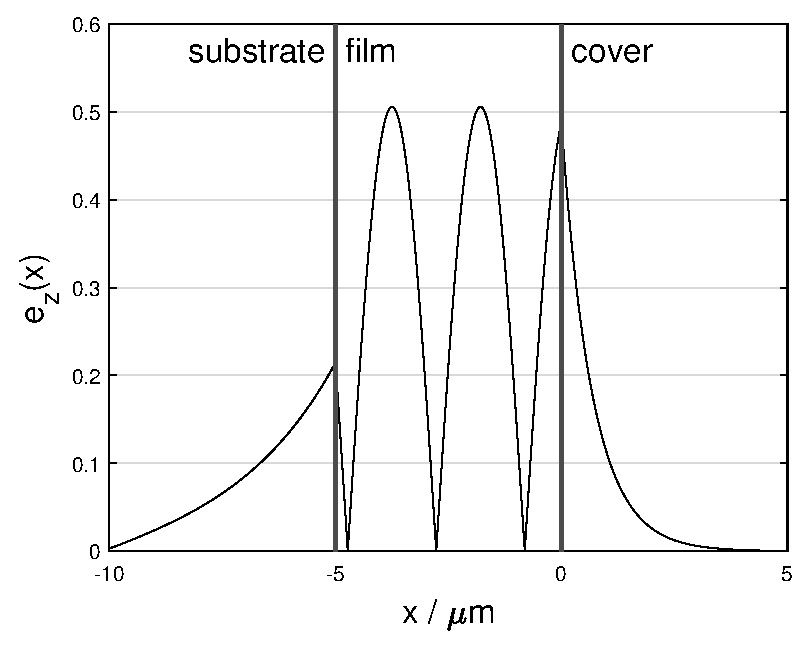
\includegraphics[width=.22\columnwidth]{Assignment-1-Problem-1-WaveGuide-2-ModalAnalysis-Mode-6-Ez.eps} \\ \hline
    \end{longtable}
    \end{itemize}
\end{sol}
\end{document}